\chapter{علم الغدد الصماء والاستتباب}\label{ch:b3:endocrinology}

في صيف عام 1921 ربط شابان في مختبر حارّ بتورنتو قنوات
البنكرياس عند كلاب، وانتظرا ذبول النسيج الهضمي، وطحنا ما
بقي، وحقنا المستخلَص في كلب جُعل سكريًا باستئصال بنكرياسه.
فهبط سكر دمه. وبحلول كانون الثاني كان صبي في الرابعة عشرة
يموت من السكري في مستشفى تورنتو العام يتلقى المستخلَص، وفي
غضون أسابيع صار يأكل ويمشي ويكتسب وزنًا؛ وعاش ثلاث عشرة سنة
أخرى. والمادة، وهي \omterm{def:b3:endocrinology:glucose}{الأنسولين}، ببتيد من واحد وخمسين حمضًا
أمينيًا تفرزه واحد في المئة من البنكرياس في الدم، حيث يخبر
عند تركيز بضع مئات من البيكومولات كلَّ خلية عضلية وشحمية في
الجسم بما تفعل بسكر الوجبة الأخيرة. وهذا الفصل عن مثل هؤلاء
الرسل: ما هم، وكيف تعرف خلية لم تلقَ الغدة قط ما يعنيه
الرسول، وكيف تُحكَم الغدد نفسها في تراتب من عرى التغذية
الراجعة، وكيف يبقي الجهاز كله غلوكوز الدم وملحه وكالسيومه
وحرارته في حدود بضع في المئة مدى العمر --- وماذا يحدث، في
العيادة، حين تخفق عروة منها.

\section{الهرمونات ومستقبلاتها}

\begin{definition}[الهرمون]\label{def:b3:endocrinology:hormone}
\index{هرمون}\index{غدة صماء}\index{إفراز مجاور}\index{هرمون ستيرويدي}\index{هرمون ببتيدي}\index{مستقبل نووي}
\emph{الهرمون} مادة تطلقها خلية في الدم فتعمل على خلايا
بعيدة تحمل مستقبلها؛ وأما الإشارة \emph{المجاورة} فتعمل على
الجيران، و\emph{الذاتية} على الخلية التي صنعتها، والهرمون
العصبي يطلقه عصبون في الدم. و\emph{الغدد الصماء} التقليدية
--- \omterm{def:b3:endocrinology:axes}{النخامى}، والدرق، وجارات الدرق، والكظران، وجزر البنكرياس،
والمناسل --- انضم إليها القلب (بالببتيد المدر للصوديوم)،
والكلية (بالإريثروبويتين)، والشحم (باللبتين)، والأمعاء
(باثني عشر ببتيدًا)، والعظم. والهرمونات كيميائيًا ثلاثة
أضرب، والكيمياء تحدد الآلية. فإن \emph{الهرمونات الببتيدية
والبروتينية} (\omterm{def:b3:endocrinology:glucose}{الأنسولين}، وهرمون النمو، وهرمونات \omterm{def:b3:endocrinology:axes}{النخامى})
تُصنع على الريبوزومات، وتُخزَّن في حبيبات، وتُطلق بالإفراغ
الخلوي، وتسير حرة في البلازما، ولا تقدر على عبور الأغشية،
وتعمل على مستقبلات عند سطح الخلية --- مقترنة بالبروتين G أو
موصولة بكيناز --- عبر رسل ثوانٍ، في غضون ثوانٍ إلى دقائق؛
وأعمار نصفها دقائق. و\emph{الستيرويدات} (الكورتيزول،
\omterm{def:b3:renal-osmoregulation:controls}{والألدوستيرون}، والإستروجينات، والتستوستيرون، \omterm{def:b3:endocrinology:calcium}{والفيتامين D} شبه
الستيرويدي) تُصنع من الكولسترول عند الحاجة، ولا تُخزَّن،
وتسير مرتبطة ببروتينات حاملة، وتعبر الأغشية، وترتبط
\emph{بمستقبلات نووية} هي نفسها عوامل استنساخ: فآثارها تأخذ
ساعات وتدوم أيامًا. و\emph{الأمينات} بين الاثنين:
فالأدرينالين يعمل عند السطح في غضون ثانية؛ وأما هرمونا
الدرق، وإن كانا مشتقي حمض أميني، فيعملان على مستقبلات نووية
كالستيرويدات. والهرمون لا يعني شيئًا بنفسه: فالأدرينالين
نفسه يوسّع وعاءً ويقبض آخر لأن عضلتيهما الملساوين تحملان
أنماطًا مختلفة من المستقبِلات، والكورتيزول نفسه يرفع غلوكوز
الدم في الكبد ويكبت \omterm{def:b3:adaptive-immunity:lymphocytes}{لمفاوية} لأن \omterm{def:b3:chromatin-epigenetics:nucleosome}{صبغين} الخليتين يعرض على
مستقبله مورّثات مختلفة.
\end{definition}

\begin{omfigure}
\begin{tikzpicture}[every node/.style={font=\scriptsize}, >=stealth]
  % peptide pathway
  \draw[thick, omDef, fill=omDef!10] (0,0) rectangle (5.2,3.4);
  \node[above] at (2.6,3.4) {هرمون ببتيدي أو أميني --- مستقبل سطحي};
  \draw[thick, omDef] (0,2.6) -- (5.2,2.6); \node[left, font=\tiny] at (5.2,2.75) {الغشاء};
  \node[circle, fill=omThm!60, inner sep=2pt, label={[font=\tiny]right:هرمون}] (h1) at (1.4,3.1) {};
  \draw[thick, omDef!80!black, fill=omDef!40] (1.1,2.3) rectangle (1.7,2.9); \node[below, font=\tiny] at (1.4,2.3) {المستقبل};
  \draw[->, thick] (2.0,2.1) -- (3.0,2.1) node[right, align=left, font=\tiny] {بروتين G أو\\فعالية كينازية};
  \draw[->, thick] (2.6,1.75) -- (2.6,1.25) node[below, align=center, font=\tiny] {cAMP، وCa$^{2+}$، وIP$_3$ أو\\شلال فسفرة};
  \draw[->, thick] (2.6,0.55) -- (2.6,0.25) node[below=-2pt, font=\tiny] {تُشغَّل إنزيمات: ثوانٍ إلى دقائق};
  % steroid pathway
  \draw[thick, omProp, fill=omProp!10] (6.4,0) rectangle (11.6,3.4);
  \node[above] at (9.0,3.4) {هرمون ستيرويدي أو درقي --- مستقبل نووي};
  \draw[thick, omProp] (6.4,2.6) -- (11.6,2.6);
  \node[circle, fill=omMeth!70, inner sep=2pt, label={[font=\tiny]right:هرمون على حامل}] (h2) at (7.6,3.1) {};
  \draw[->, thick] (7.6,2.95) -- (7.6,2.2) node[below, font=\tiny] {ينتشر عبره};
  \draw[->, thick] (7.9,1.85) -- (9.0,1.5); \draw[thick, omProp!80!black, fill=omProp!35] (8.8,1.0) rectangle (9.6,1.7); \node[right, align=left, font=\tiny] at (9.65,1.35) {معقد الهرمون\\والمستقبل، وهو\\عامل استنساخ};
  \draw[thick, omProp] (7.0,0.2) rectangle (11.0,0.8); \node[font=\tiny] at (9.0,0.5) {النواة: مورّثات تُشغَّل أو تُطفأ --- ساعات إلى أيام};
  \draw[->, thick] (9.2,1.0) -- (9.2,0.82);
\end{tikzpicture}

{\small طريقتان لسماع \omterm{def:b3:endocrinology:hormone}{هرمون}. فالهرمونات المنحلّة في الماء
تقف عند السطح وتعمل عبر رسل ثوانٍ، سريعةً قصيرة؛ والمنحلّة
في الشحم تدخل، وترتبط بمستقبل هو عامل استنساخ، فتغيّر ما
تصنعه الخلية، ببطء ولزمن طويل.}
\end{omfigure}

\begin{proposition}[الجرعة والاستجابة]\label{prop:b3:endocrinology:dose}
\index{منحنى الجرعة والاستجابة}\index{مستقبلات فائضة}\index{تنظيم نازل}
خلية فيها $R$ مستقبلًا ثابت تفككها $K_{d}$ في تركيز هرموني
$H$ يكون مشغولًا منها $R\,H/(K_{d} + H)$، وترتفع الاستجابة
عادةً مع الإشغال على منحنٍ سيني على محور جرعة لوغاريتمي،
نصف أقصاها عند $\text{EC}_{50}$ كثيرًا ما يقع دون $K_{d}$
بكثير: فإشغال بضع في المئة يعطي استجابة كاملة، لأن الإشارة
تُضخَّم فيما بعد (فمستقبل واحد يفعّل بروتينات G كثيرة،
وكيناز واحد يفسفر ركائز كثيرة)، والفائض من \emph{المستقبِلات
الفائضة} ينقل المنحني يسارًا ويجعل الخلية حساسة للجرعات
المنخفضة. والخلية تنغّم حساسيتها هي: فالتعرض المطوَّل \omterm{def:b3:endocrinology:hormone}{لهرمون}
يزيل مستقبلاته عن السطح (\emph{\omterm{prop:b3:endocrinology:dose}{التنظيم النازل}})، وهي الآلية
التي يفلّ بها \omterm{def:b3:endocrinology:glucose}{أنسولين} مرتفع باستمرار أثرَ \omterm{def:b3:endocrinology:glucose}{الأنسولين} نفسه؛
والحرمان يزيدها. وتدور الهرمونات عند $10^{-12}$ إلى
$10^{-9}$ مولاري --- أي أدنى من معظم المستقلبات بألف إلى
مليون ضعف --- ولذلك يجب أن ترتبط بها المستقبِلات بألفة
نانومولارية، ولذلك احتاج قياسها إلى طريقة جديدة.
\end{proposition}
\begin{proof}
الإشغال هو متساوي حرارة فعل الكتلة لموقع ربط واحد. فإذا
تشبعت الاستجابة حين يُشغَل $n \ll R$ مستقبلًا، كانت نصف
أقصاها حين يكون $R H/(K_{d} + H) = n/2$، أي $H = K_{d}\,
(n/2)/(R - n/2) \approx K_{d}\, n/(2R) \ll K_{d}$: فتهبط EC$_{50}$
تناسبًا مع فائض المستقبِلات. وفقدان المستقبِلات يرفعها، وهو
أثر \omterm{prop:b3:endocrinology:dose}{التنظيم النازل} على المنحني.
\end{proof}

\begin{method}[المقايسة المناعية الإشعاعية]\label{met:b3:endocrinology:ria}
\index{مقايسة مناعية إشعاعية}\index{مقايسة مناعية}
لقياس \omterm{def:b3:endocrinology:hormone}{هرمون} عند تركيز بيكومولاري (يالو وبيرسون، 1959): (1)
استنبت ضدًا له؛ (2) اخلط مقدارًا صغيرًا ثابتًا من \omterm{def:b3:adaptive-immunity:antibody}{الضد}
بمقدار ثابت من \omterm{def:b3:endocrinology:hormone}{الهرمون} الموسوم إشعاعيًا، وأضف العينة؛ (3)
ينافس \omterm{def:b3:endocrinology:hormone}{الهرمون} غير الموسوم في العينة الهرمونَ الموسوم على
مواقع \omterm{def:b3:adaptive-immunity:antibody}{الضد}، فكلما زاد \omterm{def:b3:endocrinology:hormone}{الهرمون} في العينة قلّ الموسوم
المرتبط؛ (4) افصل الموسوم المرتبط عن الحر وعُدّ؛ (5) اقرأ
تركيز العينة من منحنٍ معياري صُنع بمقادير معلومة. وخلَفُها
يستبدل بالنظير إنزيمًا أو مضيئًا ويستعمل ضدين (``شطيرة'')
لكسب النوعية؛ وهي تقيس كل \omterm{def:b3:endocrinology:hormone}{هرمون} في هذا الفصل من قطرة دم،
وقد جعلت علم الغدد الصماء علمًا كميًا.
\end{method}

\section{التراتب: الوطاء والنخامى}

\begin{definition}[المحاور]\label{def:b3:endocrinology:axes}
\index{وطاء}\index{نخامى}\index{جهاز بابي}\index{هرمون محرِّر}\index{هرمون موجِّه}\index{تغذية راجعة سالبة}
\emph{الوطاء}، وهو بضعة غرامات من الدماغ فوق النخامى، يحوّل
المعلومة العصبية --- الكرب، والبرد، وطول النهار، \omterm{def:b3:renal-osmoregulation:problem}{وأسمولية}
الدم وغلوكوزه --- إلى أوامر هرمونية. فخلاياه المفرزة عصبيًا
تطلق \emph{هرمونات محرِّرة} (ببتيدات: CRH، وTRH، وGnRH،
وGHRH، والمثبط سوماتوستاتين؛ والدوبامين للبرولاكتين) في
\emph{جهاز بابي} خاص من الأوعية يحملها، غير مخففة، سنتيمترًا
واحدًا نزولًا إلى \emph{النخامى الأمامية}، فتستجيب خلاياها
\emph{بهرمونات موجِّهة}: ACTH إلى قشر الكظر، وTSH إلى الدرق،
وLH وFSH إلى المناسل، \omterm{def:b3:endocrinology:hormone}{وهرمون} النمو إلى الكبد والنسج،
والبرولاكتين إلى الثدي. وهرمونات الغدد الهدف --- الكورتيزول،
والثيروكسين، والستيرويدات الجنسية --- تتغذى راجعةً على
النخامى والوطاء معًا فتطفئ أوامرها هي: أي \emph{تغذية راجعة
سالبة}، في ثلاث طبقات. وأما \emph{النخامى الخلفية} فليست
غدة بل نهايات محاوير عصبونات وطائية، تطلق الفازوبريسين
والأوكسيتوسين في الدم مباشرةً. ولكل محور حركياته: فمحور
الدرق بطيء ثابت، يحفظ \omterm{thm:b3:endocrinology:loop}{نقطة ضبط} سنين؛ ومحور الكظر نابض
ويوماوي، والكورتيزول يبلغ ذروته قبل الفجر ويُفرز في دفقات
كل ساعة؛ ومحور المناسل عند المرأة يدير دورة شهرية على تغذية
راجعة موجبة تفتقر إليها المحاور الأخرى.
\end{definition}

\begin{omfigure}
\begin{tikzpicture}[every node/.style={font=\scriptsize}, >=stealth]
  \node[draw, thick, rounded corners, fill=omDef!20, align=center, minimum width=3.2cm] (hyp) at (0,3.4) {الوطاء\\CRH، وTRH، وGnRH، وGHRH};
  \node[draw, thick, rounded corners, fill=omDef!20, align=center, minimum width=3.2cm] (pit) at (0,1.7) {النخامى الأمامية\\ACTH، وTSH، وLH/FSH، وGH};
  \node[draw, thick, rounded corners, fill=omProp!25, align=center, minimum width=3.2cm] (gl) at (0,0) {الغدة الهدف\\الكورتيزول، وT$_4$، والستيرويدات الجنسية};
  \node[draw, thick, rounded corners, fill=omMeth!25, align=center, minimum width=3.2cm] (tis) at (0,-1.7) {النسج: الآثار};
  \draw[->, very thick] (hyp) -- (pit) node[midway, right, font=\tiny] {الأوعية البابية};
  \draw[->, very thick] (pit) -- (gl) node[midway, right, font=\tiny] {الدم};
  \draw[->, very thick] (gl) -- (tis);
  \draw[-|, thick, omThm] (gl.west) -- ++(-0.9,0) |- (pit.west) node[pos=0.25, left, font=\tiny, omThm, align=right] {العروة\\القصيرة};
  \draw[-|, thick, omThm] (gl.west) ++(-0.9,0) -- ++(-0.7,0) |- (hyp.west) node[pos=0.25, left, font=\tiny, omThm, align=right] {العروة\\الطويلة};
  \node[left, align=right, font=\tiny] at (-2.0,4.4) {الدخلات: الكرب، والبرد،\\والضوء، والمستقلبات};
  \draw[->, thick] (-1.9,4.3) -- (hyp.north west);
  % right: the thyroid example with numbers
  \node[right, align=left] at (3.4,3.4) {محور الدرق: TRH $\to$ TSH $\to$ T$_4$، وT$_3$؛\\وعمر نصف T$_4$ سبعة أيام، ونقطة الضبط محفوظة سنين؛\\ولوغاريتم TSH يهبط خطيًا مع ارتفاع T$_4$ الحر};
  \node[right, align=left] at (3.4,1.7) {محور الكظر: CRH $\to$ ACTH $\to$ الكورتيزول؛\\ودفقات كل 1--2 ساعة، وذروة قبل الاستيقاظ؛\\والكرب يتجاوز التغذية الراجعة};
  \node[right, align=left] at (3.4,0) {محور المناسل: دفقات GnRH $\to$ LH، وFSH $\to$\\الإستراديول، والبروجسترون، والتستوستيرون؛\\واندفاع بتغذية راجعة موجبة مرة في الشهر};
  \node[right, align=left] at (3.4,-1.7) {محور النمو: GHRH، والسوماتوستاتين $\to$ GH $\to$\\IGF-1 من الكبد؛ ودفقات ليلًا};
\end{tikzpicture}

{\small المحاور الثلاثية الطبقات. تبلغ الهرمونات المحرِّرة
\omterm{def:b3:endocrinology:axes}{النخامى} عبر الأوعية البابية؛ وتأمر \omterm{def:b3:endocrinology:axes}{النخامى} غدةً؛ ويطفئ \omterm{def:b3:endocrinology:hormone}{هرمون}
الغدة الطبقتين الأعلى معًا. ولكل محور إيقاعه وإخفاقاته.}
\end{omfigure}

\begin{proof}[شواهد]
خصى برتولد (1849) ديكةً، فأضاعت عرفها وصياحها وشراستها؛
فلما أُعيد غرس خصية في أي موضع من البطن، بلا أعصابها،
استعادتها --- فالعضو عمل عبر الدم. وقطع هاريس (في خمسينيات
القرن العشرين) الأوعية البابية بين \omterm{def:b3:endocrinology:axes}{الوطاء} \omterm{def:b3:endocrinology:axes}{والنخامى} عند
جرذان: فكفّت \omterm{def:b3:endocrinology:axes}{النخامى}، وقد استُعيد إمدادها الدموي من مكان
آخر، عن الاستجابة للكرب وكفّ المبيضان عن الدورة؛ وزرعُ
\omterm{def:b3:endocrinology:axes}{نخامى} تحت الكلية تركها خاملة، وأما تحت \omterm{def:b3:endocrinology:axes}{الوطاء}، حيث نمت
الأوعية البابية فيها من جديد، فعملت --- فالدماغ يحكم الغدة
بعوامل محمولة في الدم، ثم عزل غيمان وشالي أولها، وهو TRH،
من ملايين وطاءات الخراف والخنازير (1969): ثلاثة أحماض
أمينية.
\end{proof}

\begin{proposition}[التغذية الراجعة والدرق اللوغاريتمي الخطي]\label{prop:b3:endocrinology:thyroid}
\index{هرمون درقي}\index{TSH}\index{قصور الدرق}\index{فرط الدرق}\index{دراق}
يلتقط الدرق اليوديد، ويصنع الثيروكسين T$_{4}$ (بأربع
يودات)، الذي تحوّله النسج إلى T$_{3}$ الفعال؛ وكلاهما يرفع
معدل الاستقلاب في كل خلية تقريبًا، ويضبط سرعة القلب، ولازم
لنماء الدماغ قبل الولادة وبعدها. وTSH من \omterm{def:b3:endocrinology:axes}{النخامى} يسوق تركيب
الغدة ونموها معًا؛ وT$_{4}$ يكبت TSH. والعلاقة في الحالة
المستقرة \emph{لوغاريتمية خطية}: فلوغاريتم TSH يهبط تناسبًا
مع T$_{4}$ الحر،
\[
\text{TSH} = \text{TSH}_{0}\,\mathrm{e}^{-\kappa\,(T_{4} - T_{4,0})},
\]
فهبوط T$_{4}$ الحر بمقدار الثلث يرفع TSH نحو عشرة أضعاف ---
ولذلك يكون TSH، لا T$_{4}$، هو الاختبار الحساس: فالغدة التي
تبدأ بالإخفاق تُظهر T$_{4}$ سويًّا يرفعه TSH بلغ أصلًا أضعاف
السويّ. وإخفاق الغدة (بالتهدم المناعي الذاتي، أو بعوز اليود)
يعطي \emph{\omterm{prop:b3:endocrinology:thyroid}{قصور الدرق}} --- برودة، وبطء، وتعب، مع TSH مرتفع،
ومع غدة متضخمة في عوز اليود إلى \emph{دُراق} بفعل TSH الذي
يعجز عن جعلها تنتج؛ وضدٌّ يحاكي TSH يعطي \emph{\omterm{prop:b3:endocrinology:thyroid}{فرط الدرق}}
(داء غريفز) بمريض حارّ سريع نحيل وTSH مكبوت إلى لا شيء، إذ
يفلت التحريض من التغذية الراجعة. والوليد الذي لا \omterm{prop:b3:endocrinology:thyroid}{هرمون درقي}
لديه تنشأ عنده إعاقة ذهنية لا رجعة فيها في غضون أشهر، ولذلك
يُقاس TSH عند كل وليد على نقطة دم.
\end{proposition}
\begin{proof}
يستجيب خرج TSH من خلية \omterm{def:b3:endocrinology:axes}{النخامى} لإشغال المستقبِل بجزيء T$_{3}$،
المتناسب هو نفسه مع T$_{4}$، واستجابة كبت استنساخي لتغيّر في
الإشغال ضربية --- إذ تكبت كل زيادة من \omterm{def:b3:endocrinology:hormone}{الهرمون} النسبة نفسها
مما بقي --- فيكون $\mathrm{d}\ln\text{TSH}/\mathrm{d}T_{4} = -\kappa$،
ومنه الأسّي. وبمطابقة $\kappa$ بحيث يرفع هبوط $T_{4}$ من
$15$ إلى \qty{10}{pmol/L} قيمة TSH من $1.5$ إلى \qty{15}{mU/L}،
يكون $\kappa = \ln 10/5 = \qty{0.46}{L/pmol}$: أي إن TSH يتضاعف
مع كل \qty{1.5}{pmol/L} تُفقد من T$_{4}$، وهو التضخيم الذي
يجعله الاختبار الحساس.
\end{proof}

\begin{omfigure}
\begin{tikzpicture}
\begin{semilogyaxis}[
  width=0.6\linewidth, height=5.6cm,
  axis x line=bottom, axis y line=left,
  xmin=4, xmax=30, ymin=0.02, ymax=200,
  xlabel={T$_4$ الحر (\unit{pmol/L})}, ylabel={TSH (\unit{mU/L})},
  xlabel style={font=\small, at={(axis description cs:0.5,-0.12)}, anchor=north}, ylabel style={font=\small},
  tick label style={font=\small}, xtick={5,10,15,20,25,30}, ytick={0.1,1,10,100},
  yticklabels={0.1,1,10,100},
  clip=false,
]
\addplot[very thick, omDef, domain=4.5:24.4, samples=60] {1.5*exp(-0.46*(x-15))};
\fill[omProp, opacity=0.15] (axis cs:10,0.4) rectangle (axis cs:20,4);
\node[font=\scriptsize, omProp!80!black, anchor=south] at (axis cs:15,4.2) {المجال المرجعي};
\node[font=\scriptsize, omThm, anchor=north west, align=left] at (axis cs:12,150) {غدة تخفق:\\TSH مرتفع، وT$_4$ لا يزال سويًّا};
\node[font=\scriptsize, omMeth!70!black, anchor=south west, align=left] at (axis cs:22,0.5) {داء غريفز:\\T$_4$ مرتفع، وTSH مكبوت};
\end{semilogyaxis}
\end{tikzpicture}

{\small \omterm{thm:b3:endocrinology:loop}{نقطة ضبط} الدرق منظورًا إليها من الخارج. لأن لوغاريتم
TSH يهبط خطيًا مع T$_4$، ينتج هبوط صغير في \omterm{def:b3:endocrinology:hormone}{الهرمون} ارتفاعًا
كبيرًا في الأمر --- \omterm{def:b3:endocrinology:axes}{فالنخامى} مضخّم لوغاريتمي لإخفاق الغدة.}
\end{omfigure}

\begin{example}[الكورتيزول: محور الكرب]\label{ex:b3:endocrinology:cortisol}
الكورتيزول، من قشر الكظر تحت ACTH، يعبّئ الوقود (الغلوكوز من
الكبد، والأحماض الأمينية من العضلة، والأحماض الدهنية من
الشحم)، ويحسّس الأوعية للأدرينالين، ويكبت \omterm{def:b3:innate-immunity:inflammation}{الالتهاب} والاستجابة
المناعية --- وهو سبب كون أقاربه الاصطناعية أشيع الأدوية
المضادة \omterm{def:b3:innate-immunity:inflammation}{للالتهاب}. وإيقاعه تضبطه الساعة: \qty{500}{nmol/L}
عند الثامنة صباحًا، وخُمس ذلك عند منتصف الليل، ودفقات كل
ساعة أو ساعتين على امتداد اليوم، إذ تشتعل عصبونات CRH
الوطائية دفقات. والكرب --- نزف، أو خمج، أو جراحة، أو خوف ---
يرفعه عشرة أضعاف في دقائق، متجاوزًا التغذية الراجعة. والقليل
منه (داء أديسون، أي تهدم قشر الكظر) يعطي وهنًا، وضغط دم
منخفضًا، وغلوكوزًا منخفضًا، وتحت الكرب انهيارًا وموتًا ما
لم يُعوَّض؛ والكثير منه (متلازمة كوشينغ: \omterm{def:b3:cancer-biology:hallmarks}{ورم} نخامي يصنع
ACTH، أو \omterm{def:b3:cancer-biology:hallmarks}{ورم} كظري، أو الأشيع، ستيرويدات موصوفة) يعطي الوجه
المدور، والجلد الرقيق، والعضلة الضامرة، والغلوكوز المرتفع،
والضغط المرتفع، والعظم الهشّ عند التعرض المطوَّل. وإيقاف شوط
طويل من الستيرويدات فجأةً خطر للسبب الذي يتنبأ به المحور:
\omterm{def:b3:endocrinology:axes}{فالوطاء} \omterm{def:b3:endocrinology:axes}{والنخامى} المكبوتان يحتاجان إلى أسابيع ليتعافيا،
والكظر، إذ لم يُحرَّض، قد ضمر.
\end{example}

\begin{omfigure}
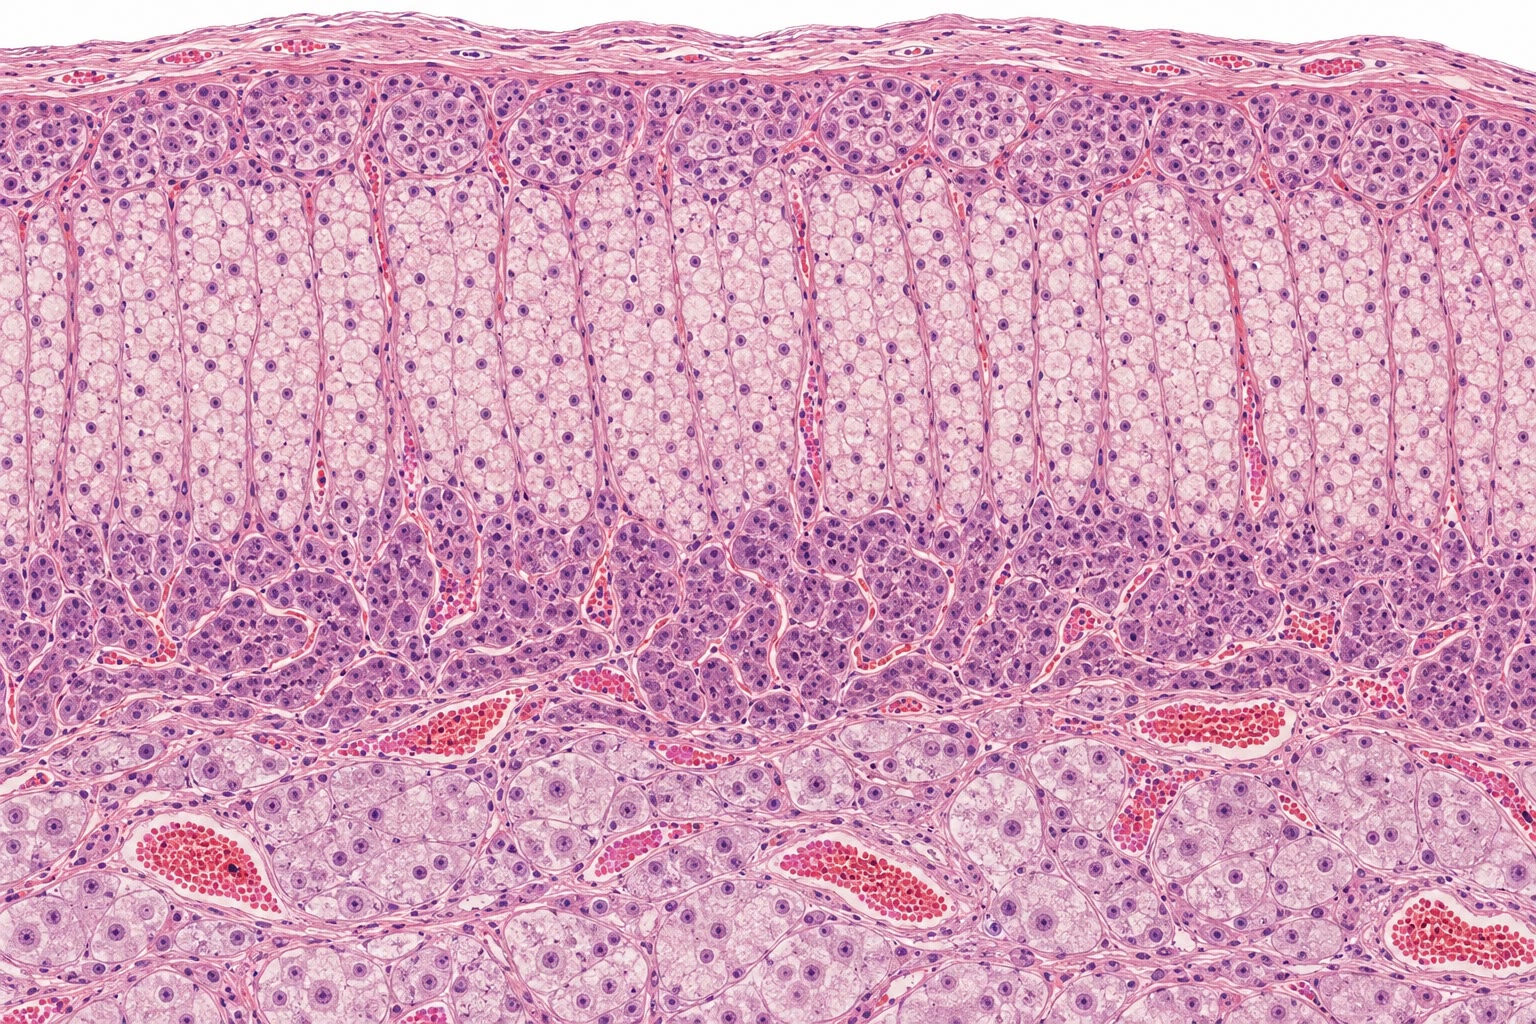
\includegraphics[width=0.5\linewidth]{images/book5/ai/b5-21-adrenal-section.jpg}\hspace{0.04\linewidth}
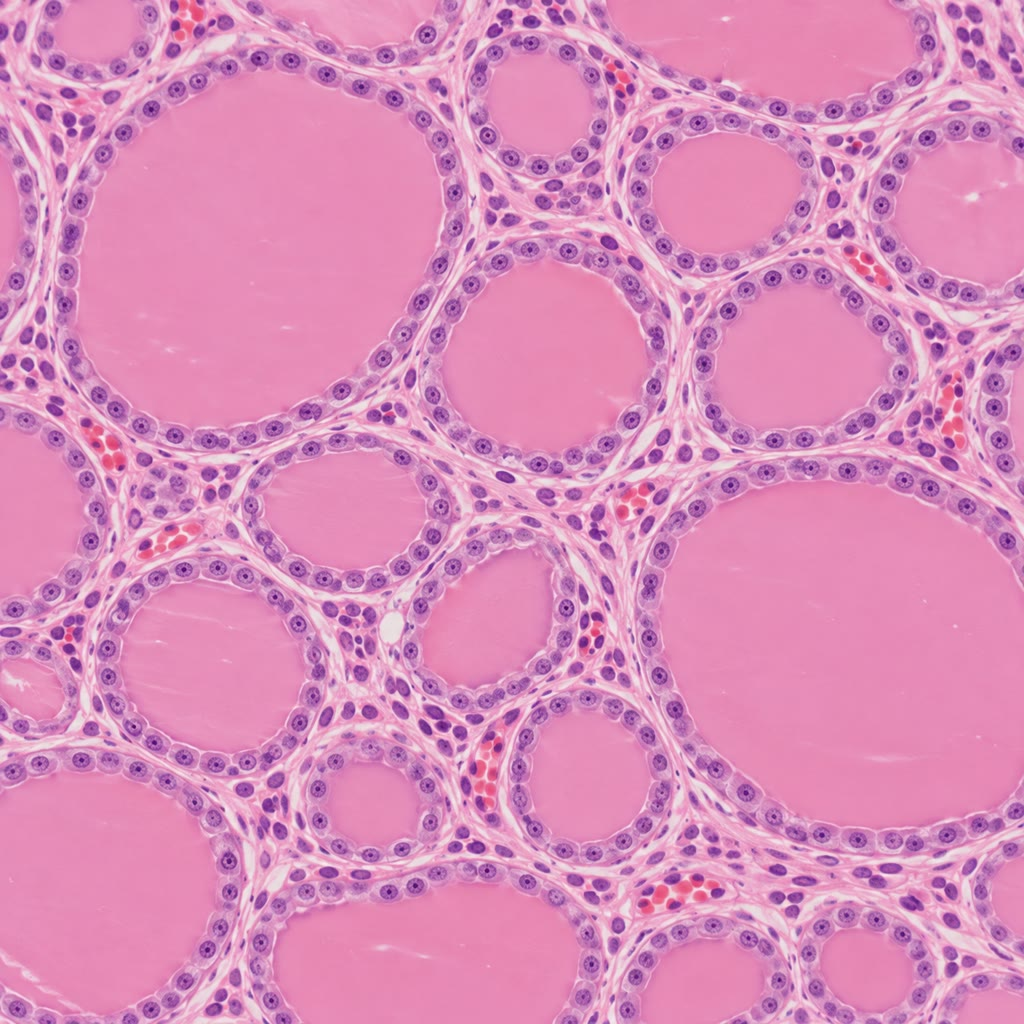
\includegraphics[width=0.36\linewidth]{images/book5/ai/b5-21-thyroid-follicles.jpg}

{\small يسارًا: الغدة الكظرية في مقطع --- القشر في مناطقه
الثلاث (\omterm{def:b3:renal-osmoregulation:controls}{الألدوستيرون} في أبعدها، والكورتيزول في المنطقة
الوسطى العريضة، والأندروجينات في أعمقها) حول لبّ من الخلايا
الأليفة للكروم المفرزة للأدرينالين، وهو عقدة ودّية بالأصل.
ويمينًا: جُرَيبات الدرق، كل واحدة كرة من الخلايا حول مخزون
من الغَرَوانيّ يحوي ما يكفي أشهرًا من \omterm{def:b3:endocrinology:hormone}{الهرمون} مرتبطًا
بالغلوبولين الدرقي.}
\end{omfigure}

\section{الغلوكوز: أشد العرى إحكامًا}

\begin{definition}[الأنسولين والغلوكاغون]\label{def:b3:endocrinology:glucose}
\index{أنسولين}\index{غلوكاغون}\index{جزيرة لانغرهانس}\index{GLUT4}\index{داء سكري}
يحوي الدم نحو \qty{5}{g} من الغلوكوز، عند \qty{5}{mmol/L}
(\qty{90}{mg/dL})، والدماغ يحرق \qty{120}{g} في اليوم ولا يقدر
على حرق شيء سواه؛ والوجبة توصل \qty{75}{g} في ساعة. و\emph{جزر
لانغرهانس}، وهي مليون عنقود من بضعة آلاف خلية متناثرة في
البنكرياس، تحمل العروة. فخلايا $\beta$ تحس الغلوكوز
باستقلابه: فغلوكوز أكثر يعني ATP أكثر، فإغلاق قناة بوتاسيوم
حساسة لجزيء ATP، فزوال استقطاب، فدخول كالسيوم، فإفراغ خلوي
\emph{للأنسولين}، وهو \omterm{def:b3:endocrinology:hormone}{هرمون ببتيدي} مشطور من سليفة واحدة.
والأنسولين يخبر العضلة والشحم بأن ينقلا الناقل \emph{GLUT4}
إلى سطحيهما ويلتقطا الغلوكوز، ويخبر الكبد بأن يخزن الغلوكوز
غليكوجينًا ويكف عن صنعه، ويخبر الشحم بأن يكف عن إطلاق
الأحماض الدهنية: فهو \omterm{def:b3:endocrinology:hormone}{هرمون} الحالة المتغذية، والوحيد الذي
يخفض غلوكوز الدم. وخلايا $\alpha$ تطلق \emph{الغلوكاغون} حين
يهبط الغلوكوز: فيهدم الكبد الغليكوجين ويصنع غلوكوزًا جديدًا
من أحماض أمينية ولاكتات. ويرفع الأدرينالين والكورتيزول
\omterm{def:b3:endocrinology:hormone}{وهرمون} النمو الغلوكوزَ أيضًا، والتكرار غير متناظر: فالجسم
يقدر على الدفاع ضد هبوط بأربعة طرق وضد ارتفاع بطريق واحد.
و\emph{الداء السكري} هو إخفاق ذلك الطريق الواحد: فالنمط 1،
أي التهدم المناعي الذاتي لخلايا $\beta$، يحتاج إلى أنسولين
من اليوم الأول؛ والنمط 2، وهو تسع حالات من عشر، يبدأ مقاومةً
من النسج للأنسولين، تُلاقى سنين بمزيد من الأنسولين، حتى
تعجز خلايا $\beta$ عن المجاراة فيرتفع الغلوكوز.
\end{definition}

\begin{theorem}[عروة الأنسولين والغلوكوز]\label{thm:b3:endocrinology:loop}
\index{كسب العروة}\index{نقطة ضبط}\index{تذبذب مخمود}
اكتب $g$ و$i$ لانحرافي غلوكوز البلازما وأنسولينها عن قيمتي
الصيام. فالغلوكوز يُصفّى بمعدل يتناسب مع فائضه هو (نجاعة
الغلوكوز $a$) ومع فائض \omterm{def:b3:endocrinology:glucose}{الأنسولين} (الحساسية $s$)؛ \omterm{def:b3:endocrinology:glucose}{والأنسولين}
يُفرز تناسبًا مع فائض الغلوكوز ($\beta$) ويُصفّى بمعدل
$\gamma$؛ ويدخل حمل $u$:
\[
\dot g = -a\,g - s\,i + u, \qquad \dot i = \beta\,g - \gamma\,i .
\]
وتحت حمل ثابت $u$ يستقر الغلوكوز عند
\[
g^{*} = \frac{u}{a}\cdot\frac{1}{1 + L}, \qquad L = \frac{s\beta}{a\gamma},
\]
فتقسم التغذية الراجعة الاضطراب الذي كان سيعانيه جسم غير
منظَّم على $1 + L$، أي \emph{\omterm{thm:b3:endocrinology:loop}{كسب العروة}} زائدًا واحدًا. وبعد
جرعة دفعية يحكم الرجوعَ القيمُ الذاتية
$\lambda = -\tfrac{a + \gamma}{2} \pm \sqrt{\tfrac{(a+\gamma)^{2}}{4} - (a\gamma + s\beta)}$:
فيكون رتيبًا إذا $s\beta < (a - \gamma)^{2}/4$، وإلا كان
تذبذبًا مخمودًا بتردد زاوي $\omega = \sqrt{a\gamma + s\beta -
(a+\gamma)^{2}/4}$ يخمد بالمقدار $\mathrm{e}^{-(a+\gamma)t/2}$ --- إذ
يهبط الغلوكوز دون قيمة صيامه قبل أن يستقر، وهي نقصُ سكر الدم
الخفيف بعد ساعتين أو ثلاث من وجبة سكرية. ومقاومة \omterm{def:b3:endocrinology:glucose}{الأنسولين}
تخفض $s$: فترتفع حالة الصيام المستقرة تحت خرج الكبد نفسه،
وتعوّض العروة بقيمة $i^{*}$ أعلى إلى أن يهبط $\beta$ في خلايا
$\beta$ أيضًا، فيخفق التعويض.
\end{theorem}
\begin{proof}
الحالة المستقرة: $\dot i = 0$ يعطي $i^{*} = \beta g^{*}/\gamma$؛
وبوضعه في $\dot g = 0$: $a g^{*} + s\beta g^{*}/\gamma = u$، ومنه $g^{*} =
u/(a + s\beta/\gamma) = (u/a)/(1 + L)$. وأما الحركيات: فمصفوفة الجملة هي
$\begin{pmatrix} -a & -s\\ \beta & -\gamma\end{pmatrix}$، أثرها
$-(a+\gamma)$ ومحددها $a\gamma + s\beta$؛ ولمعادلتها المميزة
$\lambda^{2} + (a+\gamma)\lambda + (a\gamma + s\beta) = 0$ الجذران
المذكوران. ولكليهما جزء حقيقي سالب، فحالة الصيام مستقرة؛
ويكون الجذران عقديين حين يكون المميز $(a+\gamma)^{2}
- 4(a\gamma + s\beta) = (a-\gamma)^{2} - 4s\beta$ سالبًا، وهو الشرط
المعطى، وعندئذ $g(t) = \mathrm{e}^{-(a+\gamma)t/2}(A\cos\omega t
+ B\sin\omega t)$، وهو يعبر الصفر. وأما المقاومة: فمع $u$ خرجَ
الكبد الأساسي و$s$ مخفوضًا، يهبط $L$ ويرتفع $g^{*}$ للحمل $u$
نفسه؛ ويرتفع $i^{*} = \beta g^{*}/\gamma$ معه (فرط \omterm{def:b3:endocrinology:glucose}{أنسولين}
الدم)؛ فإن هبط $\beta$ بعد ذلك، هبط $L$ أكثر وتسلق $g^{*}$ نحو $u/a$.
\end{proof}

\begin{omfigure}
\begin{tikzpicture}
\begin{axis}[
  width=0.58\linewidth, height=5.6cm,
  axis x line=bottom, axis y line=left,
  xmin=0, xmax=180, ymin=40, ymax=200,
  xlabel={الدقائق بعد جرعة غلوكوز دفعية}, ylabel={غلوكوز البلازما (mg/dL)},
  xlabel style={font=\small, at={(axis description cs:0.5,-0.12)}, anchor=north}, ylabel style={font=\small},
  tick label style={font=\small}, xtick={0,30,60,90,120,150,180}, ytick={60,90,120,150,180},
  clip=false,
]
\addplot[very thick, omDef, smooth] coordinates {(0,190) (6,165) (12,131) (18,102) (24,84) (30,77) (36,78) (42,82) (48,86) (54,89) (60,91) (66,92) (72,91) (78,91) (84,90) (90,90) (96,90) (102,90) (108,90) (114,90) (120,90) (126,90) (132,90) (138,90) (144,90) (150,90) (156,90) (162,90) (168,90) (174,90) (180,90)};
\draw[dashed, gray] (axis cs:0,90) -- (axis cs:180,90);
\node[font=\scriptsize, gray, anchor=south east] at (axis cs:180,91) {مستوى الصيام};
\node[font=\scriptsize, omDef, anchor=west, align=left] at (axis cs:75,150) {النموذج: $a = \qty{0.02}{min^{-1}}$، و$\gamma = \qty{0.1}{min^{-1}}$،\\و$s\beta = \qty{0.01}{min^{-2}}$، وكسب العروة $L = 5$؛\\وهبوط دون المستوى عند \qty{32}{min}، ودور \qty{68}{min}};
\node[font=\scriptsize, omThm, anchor=north] at (axis cs:24,70) {هبوط دون المستوى};
\end{axis}
\begin{axis}[
  at={(0.6\linewidth,0)}, anchor=south west,
  width=0.33\linewidth, height=5.6cm,
  axis x line=bottom, axis y line=left,
  xmin=0, xmax=180, ymin=0, ymax=40,
  xlabel={الدقائق}, ylabel={الأنسولين (mU/L)},
  xlabel style={font=\small, at={(axis description cs:0.5,-0.12)}, anchor=north}, ylabel style={font=\small},
  tick label style={font=\small}, xtick={0,60,120,180}, ytick={0,10,20,30,40},
]
\addplot[very thick, omProp, smooth] coordinates {(0,10.0) (6,30.0) (12,33.7) (18,28.5) (24,20.4) (30,13.4) (36,8.9) (42,7.1) (48,7.1) (54,7.9) (60,9.0) (66,9.8) (72,10.2) (78,10.4) (84,10.4) (90,10.2) (96,10.1) (102,10.0) (108,10.0) (114,9.9) (120,10.0) (126,10.0) (132,10.0) (138,10.0) (144,10.0) (150,10.0) (156,10.0) (162,10.0) (168,10.0) (174,10.0) (180,10.0)};
\draw[dashed, gray] (axis cs:0,10) -- (axis cs:180,10);
\end{axis}
\end{tikzpicture}

{\small العروة الخطية بعد جرعة دفعية ترفع الغلوكوز
\qty{100}{mg/dL}. يبلغ \omterm{def:b3:endocrinology:glucose}{الأنسولين} ذروته في غضون عشر دقائق
ويعود الغلوكوز إلى خط الأساس في عشرين، ثم يهبط دونه؛ فتغذية
راجعة قوية تعمل عبر \omterm{def:b3:endocrinology:hormone}{هرمون} له زمن تصفيته هو ترجع تذبذبًا
مخمودًا لا خمودًا بسيطًا.}
\end{omfigure}

\begin{proof}[شواهد]
استأصل فون مِرِنغ ومينكوفسكي (1889) بنكرياس كلب فأحدثا
سكريًا --- وقد وشى الذبابُ المحتشد على بوله بالسكر؛ وأما ربط
القنوات، الذي هدم النسيج الهضمي وأبقى الجزر، فلم يفعل. واستخلص
بانتنغ وبست (1921)، بتنقية كوليب، مبدأ الجزر وخفضا سكر دم
كلب سكري، ثم سكر دم ليونارد طومسون (كانون الثاني 1922).
وسلسل سانغر \omterm{def:b3:endocrinology:glucose}{الأنسولين} (1955)، وكان أول تسلسل بروتيني؛ وقاسه
يالو وبيرسون في الدم (1959) فوجدا أن سكريّي البلوغ كان
لديهم، في البداية، منه أكثر مما لدى الأصحاء --- أي مقاومة لا
عوزًا. وصنعت بكتيريا جينينتك الأنسولينَ البشري عام 1978،
وكان أول دواء مؤشَّب.
\end{proof}

\begin{omfigure}
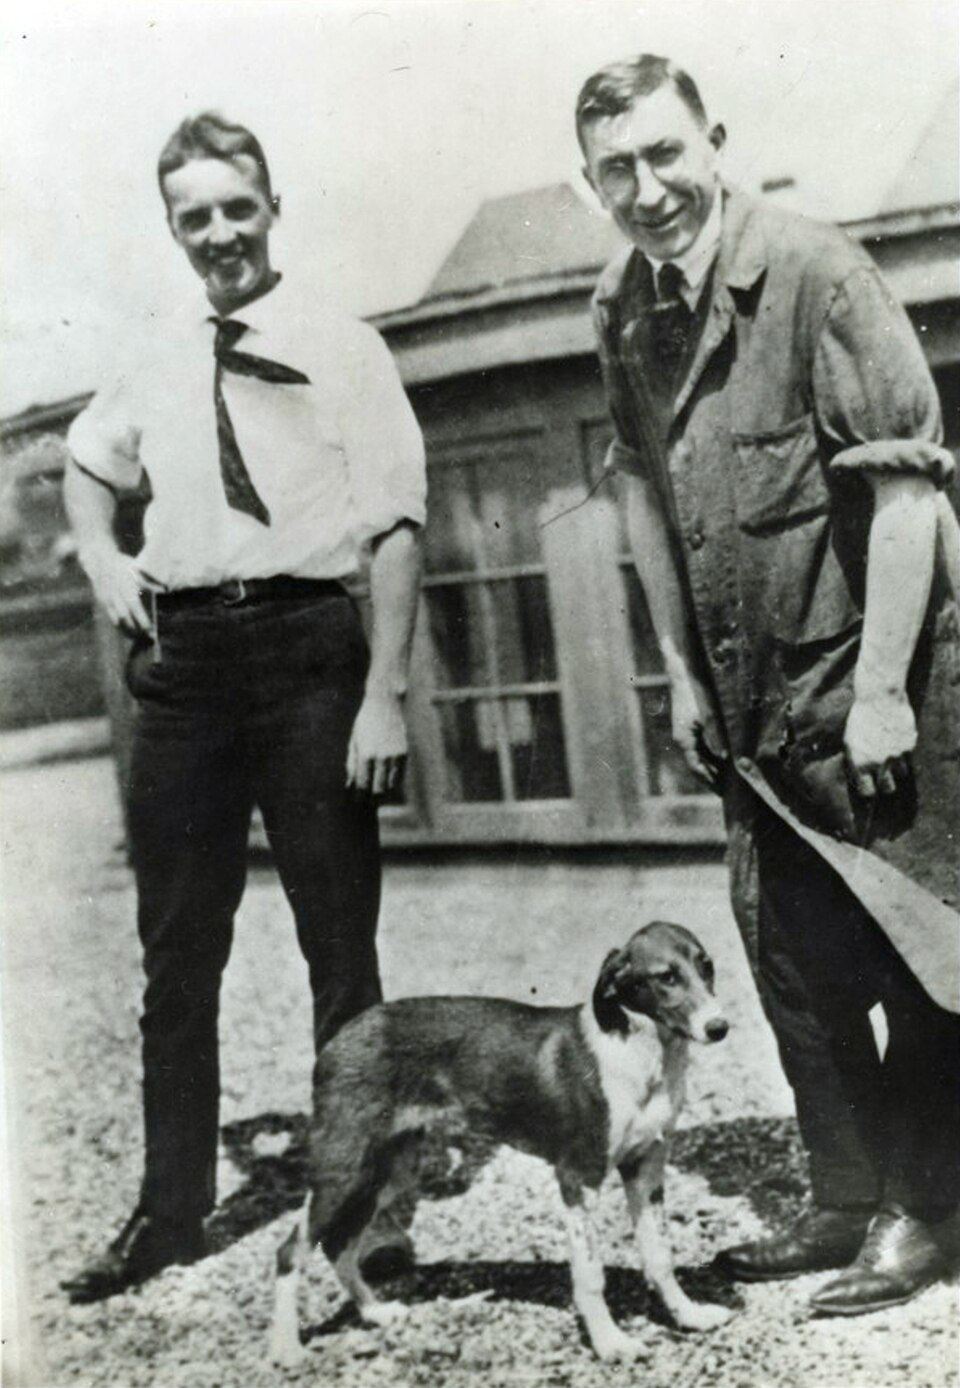
\includegraphics[width=0.42\linewidth]{images/book5/banting-best.jpg}\hspace{0.04\linewidth}
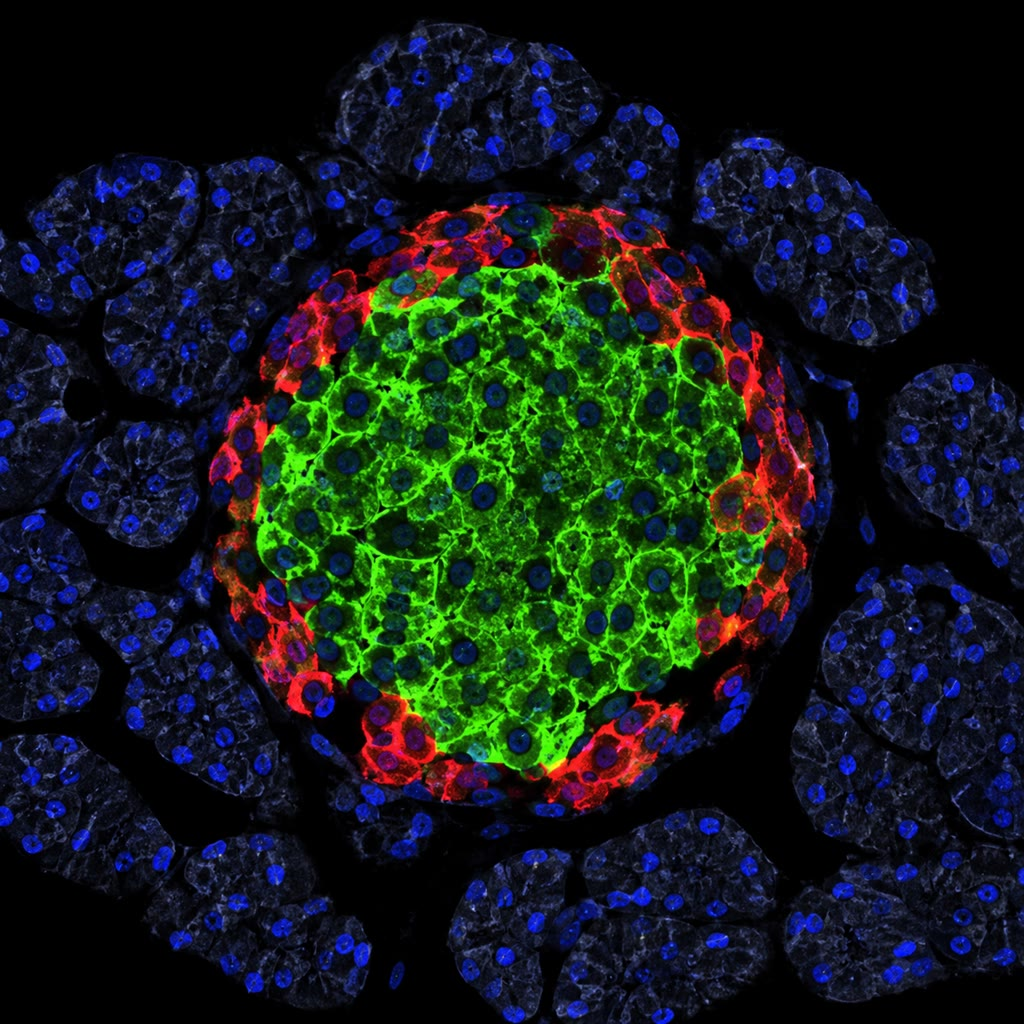
\includegraphics[width=0.42\linewidth]{images/book5/ai/b5-21-pancreatic-islet.jpg}

{\small يسارًا: فردريك بانتنغ وتشارلز بست على سطح مبنى الطب
في تورنتو، نحو عام 1924، مع أحد كلاب تجارب \omterm{def:b3:endocrinology:glucose}{الأنسولين} (صورة
في الملكية العامة). ويمينًا: \omterm{def:b3:endocrinology:glucose}{جزيرة لانغرهانس}، وخلايا $\beta$
المنتجة \omterm{def:b3:endocrinology:glucose}{للأنسولين} في قلبها، وخلايا $\alpha$ المنتجة
\omterm{def:b3:endocrinology:glucose}{للغلوكاغون} عند حافتها، في بحر من العُنَيبات الخارجية
الإفراز.}
\end{omfigure}

\begin{method}[قراءة عروة الغلوكوز عند مريض]\label{met:b3:endocrinology:ogtt}
\index{اختبار تحمل الغلوكوز}\index{HbA1c}
(1) غلوكوز البلازما صائمًا: السويّ دون \qty{5.6}{mmol/L}،
والسكري عند \qty{7.0}{mmol/L} أو فوقها في مناسبتين. (2)
\omterm{met:b3:endocrinology:ogtt}{اختبار تحمل الغلوكوز} الفموي: تُشرب \qty{75}{g} من الغلوكوز؛
وغلوكوز البلازما عند ساعتين سويّ دون \qty{7.8}{mmol/L}،
وسكري عند \qty{11.1}{mmol/L} أو فوقها --- فقيمة الساعتين تقرأ
\omterm{thm:b3:endocrinology:loop}{كسب العروة}، وقيمة الصيام تقرأ نقطة ضبطها. (3) الهيموغلوبين
المسكَّر، \emph{HbA1c}: يرتبط الغلوكوز بالهيموغلوبين ارتباطًا
لا رجعة فيه بمعدل يتناسب مع تركيزه، وتعيش الكريات الحمر 120
يومًا، فتكامل النسبة المسكَّرة متوسط الغلوكوز في الأشهر
الثلاثة الماضية بلا صيام --- والسويّ دونها \qty{5.7}{\%}،
والسكري من \qty{6.5}{\%}. (4) وللفصل بين المقاومة والعوز، قس
\omterm{def:b3:endocrinology:glucose}{الأنسولين} (أو ناتجه الجانبي الببتيد C) إلى جانبه: \omterm{def:b3:endocrinology:glucose}{فأنسولين}
مرتفع مع غلوكوز مرتفع مقاومةٌ؛ وغياب الببتيد C نمطٌ~1.
\end{method}

\section{الكالسيوم، والساعة}

\begin{definition}[استتباب الكالسيوم]\label{def:b3:endocrinology:calcium}
\index{هرمون جارات الدرق}\index{كالسيتريول}\index{فيتامين D}\index{تخلخل العظم}
يُبقى الكالسيوم المتأين في البلازما عند \qty{1.2}{mmol/L} في
حدود بضع في المئة، لأنه يحدد استثارية كل عصب وعضلة: فإن
انخفض كثيرًا اشتعلا عفويًا (تكزز)، وإن ارتفع كثيرًا صارا
خاملين. وتحس غدد جارات الدرق الأربع الكالسيوم بمستقبل سطحي
وتفرز \emph{\omterm{def:b3:endocrinology:hormone}{هرمون} جارات الدرق} (PTH) على منحنٍ سيني عكسي
حادّ: فيعبّئ PTH الكالسيوم من العظم، ويجعل الكلية تعيد
امتصاصه وتطرح الفوسفات، ويفعّل \emph{الفيتامين D} --- المصنوع
في الجلد بالأشعة فوق البنفسجية أو المأكول، المهدرَك في الكبد
ثم في الكلية إلى \emph{كالسيتريول} --- الذي يجعل الأمعاء
تمتص الكالسيوم. والعظم هو الخزان، كيلوغرام من الكالسيوم،
يُعاد بناؤه باستمرار بناقضات العظم وبانياته تحت PTH
والكالسيتريول والإستروجين والحمل. وعوز الفيتامين D يعطي
الكُساح عند الأطفال ولين العظام عند البالغين؛ وهبوط
الإستروجين عند سن اليأس يميل بإعادة البناء نحو الامتصاص
فيعطي \emph{تخلخل العظم}؛ \omterm{def:b3:cancer-biology:hallmarks}{وورم} غدي في جارة الدرق يرفع
الكالسيوم، ويذيب العظم، ويكوّن حصى الكلى --- ``عظام، وحصى،
وأنين، وتشكّ.''
\end{definition}

\begin{definition}[الساعة اليوماوية]\label{def:b3:endocrinology:clock}
\index{ساعة يوماوية}\index{نواة فوق التصالب}\index{مورّثات الساعة}\index{ميلاتونين}\index{مزامن}
تحمل كل خلية تقريبًا \emph{ساعة يوماوية}: وهي عروة استنساخ
وترجمة يشغّل فيها البروتينان CLOCK وBMAL1 المورّثتين
\emph{Per} و\emph{Cry}، فتتراكم بروتيناتهما، وتدخل النواة
بعد تأخير ساعات وتكبت استنساخها هي، ثم تُهدَم، فيرتفع الكبت
--- أي دورة في نحو أربع وعشرين ساعة، تحددها معدلات التأخير
والهدم. وتُزامَن ساعات الجسم بساعة رئيسة من عشرين ألف عصبون
في \emph{النواة فوق التصالب} في \omterm{def:b3:endocrinology:axes}{الوطاء}، وهي نفسها يضبطها
الضوء عبر صنف مخصص من الخلايا العقدية \omterm{def:b3:sensory-systems:retina}{الشبكية} (تحوي
الميلانوبسين، لا أصبغة العصيّات ولا المخاريط)، وهي تشير
بالليل إلى الجسم عبر \emph{ميلاتونين} الصنوبرية، الذي لا
يُفرز إلا في الظلام. وتجدول الساعة الكورتيزول قبل الاستيقاظ،
وأدنى حرارة للجسم عند الرابعة صباحًا، \omterm{def:b3:endocrinology:hormone}{وهرمون} النمو في أول
النوم، وحساسية \omterm{def:b3:endocrinology:glucose}{الأنسولين} أعلى صباحًا؛ والطعام والرياضة
والحرارة \emph{مزامنات} ثانوية تقدر على جذب الساعات المحيطية
بعيدًا عن المركزية، وهي وعكة عامل المناوبات ووعكة الطيران
--- ساعة كبد على توقيت ودماغ على آخر.
\end{definition}

\begin{proof}[شواهد]
فحص كونوبكا وبنزر (1971) ذبابًا طافرًا بحثًا عن إيقاعات خروج
متبدلة فوجدا ثلاثة أليلات لمورّثة واحدة، هي \emph{period}:
نهار قصير (19 ساعة)، ونهار طويل (29 ساعة)، ولا إيقاع البتة
--- أي ساعة ذات دور وراثي. ووجد هاردن وهول وروزباش (1990) أن
RNA الرسول للمورّثة \emph{period} وبروتينها يتذبذبان بتأخر بينهما،
وأن البروتين يكبت مورّثته هو: فتلك العروة. وزرع رالف وميناكر
(1990) \omterm{def:b3:endocrinology:clock}{النواة فوق التصالب} من هامستر طافر إيقاعه 20 ساعة في
هامستر سويّ هُدمت نواته هو: فسار المتلقي على 20 ساعة ---
فالدور ينتمي إلى النسيج المزروع. وفي البشر المحفوظين في مخبأ
بلا إشارات زمنية سار الإيقاع حرًّا عند أكثر قليلًا من 24
ساعة؛ وضوء ساطع مساءً أخّره، وصباحًا قدّمه.
\end{proof}

\begin{omfigure}
\begin{tikzpicture}[every node/.style={font=\scriptsize}, >=stealth]
  \node[draw, thick, rounded corners, fill=omDef!20, align=center] (cb) at (0,1.6) {CLOCK--BMAL1\\المنشِّطان};
  \node[draw, thick, rounded corners, fill=omProp!25, align=center] (pc) at (3.6,1.6) {\emph{Per}، و\emph{Cry}\\مستنسختان};
  \node[draw, thick, rounded corners, fill=omThm!20, align=center] (pr) at (3.6,-0.4) {بروتينا PER وCRY\\يتراكمان ويتثانيان};
  \node[draw, thick, rounded corners, fill=omMeth!25, align=center] (nu) at (0,-0.4) {يدخلان النواة\\بعد ساعات};
  \draw[->, thick] (cb) -- (pc) node[midway, above, font=\tiny] {ينشّطان};
  \draw[->, thick] (pc) -- (pr) node[midway, right, font=\tiny] {ترجمة، وتأخير};
  \draw[->, thick] (pr) -- (nu);
  \draw[-|, thick, omThm] (nu) -- (cb) node[midway, left, font=\tiny, omThm, align=right] {يكبتان\\منشِّطيهما\\هما};
  \draw[->, thick, gray] (nu.south) -- ++(0,-0.5) node[below, font=\tiny, gray] {يُهدمان: فيرتفع الكبت، وتبدأ الدورة من جديد $\approx$ \qty{24}{h}};
  % right: daily profile
  \begin{scope}[shift={(7.2,-1.6)}]
    \draw[->] (0,0) -- (5.6,0) node[right, font=\tiny] {الساعة};
    \draw[->] (0,0) -- (0,3.4);
    \foreach \x/\l in {0/0, 1.4/6, 2.8/12, 4.2/18, 5.6/24} { \draw (\x,0) -- (\x,-0.08) node[below, font=\tiny] {\l}; }
    \fill[gray!25] (0,0) rectangle (1.4,3.4); \fill[gray!25] (5.1,0) rectangle (5.6,3.4);
    \node[font=\tiny, gray!60!black] at (0.7,3.2) {ليل};
    \draw[very thick, omMeth!70!black, domain=0:5.6, samples=60, smooth, variable=\x] plot (\x, {1.6 + 1.2*cos(deg(2*3.1416*(\x-1.9)/5.6))});
    \node[font=\tiny, omMeth!70!black] at (3.1,3.1) {الكورتيزول: ذروة عند الثامنة صباحًا};
    \draw[very thick, omDef, domain=0:5.6, samples=60, smooth, variable=\x] plot (\x, {0.9 + 0.7*cos(deg(2*3.1416*(\x-0.7)/5.6))});
    \node[font=\tiny, omDef] at (2.7,0.18) {الميلاتونين: ليلًا فقط};
  \end{scope}
\end{tikzpicture}

{\small يسارًا: لبّ الساعة الجزيئية، وهي عروة \omterm{def:b3:endocrinology:axes}{تغذية راجعة
سالبة} بتأخير ساعات، وهو ما تحتاج إليه العروة لتتذبذب بدل أن
تستقر. ويمينًا: هرمونان تجدولهما --- الكورتيزول يرتفع قبل
الفجر ليهيئ النهار، \omterm{def:b3:endocrinology:clock}{والميلاتونين} يعلّم الليل.}
\end{omfigure}

\begin{remark}[الاستتباب تحكّمًا]\label{rem:b3:endocrinology:control}
لكل عروة في هذا الفصل الأجزاء نفسها: مجسّ (استقلاب خلية
$\beta$، ومستقبل الكالسيوم في جارة الدرق، ومستقبل \omterm{prop:b3:endocrinology:thyroid}{الهرمون
الدرقي} في \omterm{def:b3:endocrinology:axes}{النخامى})، ومتحكم يقارن \omterm{thm:b3:endocrinology:loop}{بنقطة ضبط}، \omterm{def:b3:endocrinology:hormone}{وهرمون} منفِّذ له
عمر نصفه، وتغذية راجعة تخفض الخطأ بعامل $1 + L$ لا إلى الصفر
أبدًا. والذي يختلف هو التوقيت --- ثوانٍ للأدرينالين، وساعة
\omterm{def:b3:endocrinology:glucose}{للأنسولين}، وأيام للثيروكسين، وعمر كامل للعظم --- وثمن
المساومة: فعروة سريعة بمنفِّذ متأخر تتذبذب، وعروة بطيئة تدع
الاضطراب يدوم. والعيادة ترى العرى من الخارج، عبر الأزواج
التي تقرنها التغذية الراجعة: \omterm{def:b3:endocrinology:hormone}{فهرمون} TSH مرتفع مع T$_{4}$ منخفض
غدةٌ مخفقة، وTSH مرتفع مع T$_{4}$ مرتفع \omterm{def:b3:endocrinology:axes}{نخامى} مخفقة؛
\omterm{def:b3:endocrinology:glucose}{وأنسولين} مرتفع مع غلوكوز مرتفع مقاومةٌ، \omterm{def:b3:endocrinology:glucose}{وأنسولين} منخفض مع
غلوكوز مرتفع تهدّمٌ. ولقراءة مستوى \omterm{def:b3:endocrinology:hormone}{هرمون} يجب أن يُسأل دائمًا
عمّا كان آمره يفعل.
\end{remark}

\section{تمارين}

\begin{exercise}[$\star$]\label{exo:b3:endocrinology:1}
صنّف \omterm{def:b3:endocrinology:glucose}{الأنسولين} والكورتيزول والأدرينالين والثيروكسين
والفازوبريسين بحسب الكيمياء، وموضع المستقبل، وسرعة الفعل،
وعمر النصف.
\end{exercise}

\begin{exercise}[$\star$]\label{exo:b3:endocrinology:2}
ارسم محور الدرق بتغذيته الراجعة وتنبأ بقيمتي TSH وT$_{4}$ في:
درق مهدَّم؛ \omterm{def:b3:cancer-biology:hallmarks}{وورم} نخامي يفرز TSH؛ ومريض يتناول ثيروكسينًا
أكثر مما ينبغي؛ وعوز اليود.
\end{exercise}

\begin{exercise}[$\star$]\label{exo:b3:endocrinology:3}
لماذا للجسم أربعة هرمونات ترفع غلوكوز الدم وواحد فقط يخفضه؟
وبماذا يتنبأ ذلك عن الخطر النسبي \omterm{def:b3:endocrinology:glucose}{لأنسولين} أكثر مما ينبغي
\omterm{def:b3:endocrinology:glucose}{وأنسولين} أقل مما ينبغي؟
\end{exercise}

\begin{exercise}[$\star$]\label{exo:b3:endocrinology:4}
ما \omterm{def:b3:endocrinology:clock}{المزامن}؟ اذكر ثلاثة، وقل أيها تستعمل الساعة الرئيسة،
واشرح ماذا يحدث لمسافر يعبر ثماني مناطق زمنية.
\end{exercise}

\begin{exercise}[$\star\star$]\label{exo:b3:endocrinology:5}
خلية فيها \num{20000} مستقبل عند $K_{d} = \qty{1}{nM}$ وتستجيب
استجابة قصوى حين يُشغَل \num{500} منها. جِد EC$_{50}$. وبعد
أسبوع من \omterm{def:b3:endocrinology:hormone}{هرمون} مرتفع صار في الخلية \num{2000} مستقبل: فما
EC$_{50}$ الجديدة؟ وفسّر ذلك لمقاومة \omterm{def:b3:endocrinology:glucose}{الأنسولين}.
\end{exercise}

\begin{exercise}[$\star\star$]\label{exo:b3:endocrinology:6}
عند $\kappa = \qty{0.46}{L/pmol}$ وTSH سويّ قدره \qty{1.5}{mU/L}
عند T$_{4}$ حر قدره \qty{15}{pmol/L}، احسب TSH حين يكون
T$_{4}$ عند $13$ و$11$ و$9$ و\qty{25}{pmol/L}. وعند أي منها
يكون T$_{4}$ لا يزال ضمن مجال مرجعي \qtyrange{10}{20}{pmol/L}
بينما TSH خارج \qtyrange{0.4}{4}{mU/L}؟
\end{exercise}

\begin{exercise}[$\star\star$]\label{exo:b3:endocrinology:7}
في عروة \cref{thm:b3:endocrinology:loop} عند $a = \qty{0.02}{min^{-1}}$،
و$\gamma = \qty{0.1}{min^{-1}}$، و$\beta = \qty{0.05}{mU\,L^{-1}\,min^{-1}}$
لكل mg/dL، و$s = \qty{0.2}{mg\,dL^{-1}\,min^{-1}}$ لكل mU/L، احسب
\omterm{thm:b3:endocrinology:loop}{كسب العروة}، وفائض الغلوكوز المستقر تحت حمل ثابت قدره
\qty{2}{mg/dL/min}، والمقدار نفسه بلا تغذية راجعة، وفائض
\omterm{def:b3:endocrinology:glucose}{الأنسولين} المستقر.
\end{exercise}

\begin{exercise}[$\star\star$]\label{exo:b3:endocrinology:8}
بالمُعاملات نفسها: هل يكون الرجوع بعد جرعة دفعية تذبذبيًا؟
احسب الدور والزمن اللازم لهبوط السعة بعامل $\mathrm{e}$. ثم
نصّف $s$ (مقاومة \omterm{def:b3:endocrinology:glucose}{الأنسولين}): أعد حسابهما وحساب \omterm{thm:b3:endocrinology:loop}{كسب العروة}
الجديد.
\end{exercise}

\begin{exercise}[$\star\star$]\label{exo:b3:endocrinology:9}
عمر نصف الكورتيزول \qty{80}{min}. مريض على \qty{40}{mg} من
البريدنيزولون يوميًا سنةً يتوقف فجأةً. اشرح، طبقةً طبقة،
لماذا قد ينهار تحت خمج طفيف بعد ثلاثة أيام، وماذا كان
المحور سيُظهر لو قيس (ACTH، والكورتيزول، والاستجابة لحقن
ACTH).
\end{exercise}

\begin{exercise}[$\star\star\star$]\label{exo:b3:endocrinology:10}
بيّن أن \omterm{def:b3:endocrinology:axes}{تغذية راجعة سالبة} بمتغير واحد $\dot x = f(x)$ عند
$f' < 0$ لا تقدر على التذبذب، بينما تقدر عليه عروة المبرهنة
ذات المتغيرين، واشرح بالكلام لماذا تحتاج الساعة إلى تأخير
ساعات بين الاستنساخ والكبت لتنتج دورًا مدته 24 ساعة. وماذا
كان سيحدث للدور لو هُدم PER بسرعة مضاعفة؟
\end{exercise}

\begin{exercise}[$\star\star\star$]\label{exo:b3:endocrinology:11}
يتبع \omterm{def:b3:endocrinology:calcium}{هرمون جارات الدرق} العلاقة $\text{PTH} = P_{\max}/(1 +
\mathrm{e}^{k(\text{Ca} - \text{Ca}_{0})})$ عند $\text{Ca}_{0} =
\qty{1.2}{mmol/L}$ و$k = \qty{20}{L/mmol}$. احسب PTH كنسبة من
الأقصى عند Ca $= 1.10$ و$1.15$ و$1.20$ و$1.25$ و\qty{1.30}{mmol/L}،
والميل عند \omterm{thm:b3:endocrinology:loop}{نقطة الضبط}، واشرح لماذا يُطلب مثل هذا الانحدار
للكالسيوم ويكون خطرًا للغلوكوز.
\end{exercise}

\begin{exercise}[$\star\star\star$]\label{exo:b3:endocrinology:12}
يرتبط الغلوكوز بالهيموغلوبين بمعدل $k\,G$ في وحدة الزمن،
و$k$ بحيث يعطي متوسط غلوكوز قدره \qty{5.5}{mmol/L} تسكّرًا
قدره \qty{5}{\%} على مدى عمر كرية حمراء البالغ 120 يومًا.
استنتج HbA1c دالةً لمتوسط الغلوكوز، والقيمة عند
\qty{10}{mmol/L}، واشرح لماذا يكون HbA1c عند مريض بفقر دم
انحلالي (كرياته تعيش 60 يومًا) منخفضًا انخفاضًا مضلِّلًا.
\end{exercise}

\section{مسألة: السكر في الدم}

\begin{problem}[{مسألة نهاية الأسبوع --- اختبار تحمل غلوكوز
يُقرأ عبر عروة \omterm{def:b3:endocrinology:glucose}{الأنسولين} والغلوكوز الخطية: توزع جرعة
\qty{75}{g}، \omterm{thm:b3:endocrinology:loop}{وكسب العروة} والرجوع المخمود، وما تفعله المقاومة
وإخفاق خلايا $\beta$ \omterm{thm:b3:endocrinology:loop}{بنقطة ضبط} الصيام، وتشخيص من الأرقام،
ومحور الدرق بجانبه، وتُختم \omterm{thm:b3:endocrinology:loop}{بكسب العروة}، وبزمن الرجوع،
وبغلوكوز الصيام في العروة المخفقة}]
\label{pb:b3:endocrinology:1}
المعطيات: بالغ سليم، وحجم توزع الغلوكوز \qty{15}{L}، وغلوكوز
الصيام \qty{90}{mg/dL} (\qty{5}{mmol/L})، \omterm{def:b3:endocrinology:glucose}{وأنسولين} الصيام
\qty{10}{mU/L}. ومُعاملات العروة: $a = \qty{0.02}{min^{-1}}$، و$\gamma =
\qty{0.1}{min^{-1}}$، و$\beta = 0.05$ (mU/L لكل دقيقة لكل mg/dL)، و$s = 0.2$
(mg/dL لكل دقيقة لكل mU/L). وخرج الكبد الغلوكوزي الأساسي $u_{0} =
\qty{2}{mg/dL/min}$ (وهو متوازن أصلًا في حالة الصيام مع تخلص
الصيام). وجرعة فموية قدرها \qty{75}{g} تُمتص على مدى ساعة.
والدرق: $\text{TSH} = 1.5\,\mathrm{e}^{-0.46(T_{4} - 15)}$ بوحدة mU/L.
والكتلة المولية للغلوكوز \qty{180}{g/mol}.

\medskip
\noindent\textbf{الجزء الأول --- الجرعة.}
\begin{enumerate}
  \item عبّر عن غلوكوز الصيام بالميلي مول في اللتر وتحقق من
        التحويل من mg/dL. وكم غرامًا من الغلوكوز في حجم التوزع عند
        الصيام؟
  \item لو ظهرت \qty{75}{g} كلها دفعةً واحدة في \qty{15}{L}،
        فبكم يرتفع الغلوكوز (بالميليغرام في الديسيلتر وبالميلي
        مول في اللتر)؟
        ولماذا تقصّر الذروة الحقيقية، وهي نحو \qty{60}{mg/dL}
        فوق الصيام، عن ذلك كثيرًا؟
  \item إذا امتُصت على مدى \qty{60}{min}، فبأي معدل تدخل
        الجرعة بوحدة mg/dL في الدقيقة؟ وقارن ذلك بالمقدار
        $u_{0}$.
  \item بلا أي استجابة أنسولينية ($s = 0$)، يخضع الغلوكوز
        للعلاقة $\dot
        g = -a g + u$. فما الفائض المستقر تحت
        معدل الامتصاص، وما ثابت زمن الاقتراب؟ وأين سيكون
        الغلوكوز بعد ساعة؟
  \item مع العروة، احسب $L$ والفائض المستقر تحت المعدل نفسه.
        وقارن ذلك بالسؤال~4.
  \item اشرح لماذا يُحمى الدماغ من الجهتين: ماذا يحتاج،
        وماذا يفعل الغلوكوز الزائد بالنسج على مدى سنين.
\end{enumerate}

\medskip
\noindent\textbf{الجزء الثاني --- الرجوع.}
\begin{enumerate}[resume]
  \item اكتب المعادلة المميزة للعروة واحسب الأثر والمحدد
        والمميز.
  \item احسب $\omega$ ودور \omterm{thm:b3:endocrinology:loop}{التذبذب المخمود}، وزمن الخمود
        $2/(a + \gamma)$.
  \item انطلاقًا من فائض قدره \qty{100}{mg/dL} \omterm{def:b3:endocrinology:glucose}{والأنسولين} عند
        قيمة صيامه، يكون الحل $g(t) = 100\,\mathrm{e}^{-0.06t}
        (\cos\omega t + c\sin\omega t)$. جِد $c$ من $\dot g(0) = -a\cdot
        100$.
  \item متى يعود الغلوكوز أول مرة إلى قيمة الصيام (أول صفر
        للدالة $g$)؟ وقدّر الهبوط دون المستوى عند أول نهاية
        صغرى.
  \item \omterm{def:b3:endocrinology:glucose}{الأنسولين}: للدالة $i(t)$ الأسّي نفسه والتردد نفسه.
        احتجّ من $\dot i = \beta g - \gamma i$ لأن ذروته تأتي
        بعد أن يبدأ الغلوكوز بالهبوط وقبل أن يبلغ الغلوكوز
        قيمة الصيام.
  \item لماذا يُظهر اختبار تحمل حقيقي، بامتصاص على مدى ساعة
        لا بجرعة دفعية، ذروةً عند 30--60 دقيقة ورجوعًا في
        غضون ساعتين، وهبوطًا خفيفًا فقط عند ثلاث؟
\end{enumerate}

\medskip
\noindent\textbf{الجزء الثالث --- حين تخفق العروة.}
\begin{enumerate}[resume]
  \item تنصّف مقاومة \omterm{def:b3:endocrinology:glucose}{الأنسولين} قيمة $s$. فما $L$ الجديد؟
        وخرج الكبد $u_{0}$ تلاقيه الآن حالة صيام مستقرة
        جديدة: فباستعمال $g^{*} = (u_{0}/a)/(1
        + L)$ فائضًا فوق خط أساس غير منظَّم مثالي، جِد بكم
        يرتفع غلوكوز الصيام بالنسبة إلى الحالة السليمة (احسب
        قيمتي $g^{*}$ واطرح).
  \item \omterm{def:b3:endocrinology:glucose}{أنسولين} الصيام في الحالة المقاومة: احسب $i^{*} = \beta
        g^{*}/\gamma$ للحالتين والنسبة بينهما. وماذا تسمي
        العيادة ذلك؟
  \item ثم تخفق خلايا $\beta$: فيهبط $\beta$ إلى الخُمس أيضًا.
        فما $L$ الجديد، وما فائض الصيام الجديد؟ حوّله إلى الميلي
        مول في اللتر وقارنه بالعتبة السكرية \qty{7}{mmol/L}.
  \item هل يبقى الرجوع تذبذبيًا في حالة السؤال~15؟ احسب
        المميز وثابت زمن أبطأ نمط.
  \item مريض غلوكوز صيامه \qty{8}{mmol/L}، \omterm{def:b3:endocrinology:glucose}{وأنسولين} صيامه
        \qty{30}{mU/L}، وقيمة الساعتين \qty{13}{mmol/L}. شخّص
        النمط والآلية من الأزواج.
  \item وآخر غلوكوز صيامه \qty{15}{mmol/L}، والببتيد C غير
        قابل للكشف، وقد فقد \qty{8}{kg} في شهرين. شخّص، واشرح
        نقص الوزن من حيث ما تفعله النسج بلا \omterm{def:b3:endocrinology:glucose}{أنسولين}.
  \item الهيموغلوبين المسكَّر: إذا كان متوسط غلوكوز المريض
        الأول \qty{9}{mmol/L}، وكانت \qty{5.5}{mmol/L} تعطي
        \qty{5}{\%}، فقدّر HbA1c عنده بفرض التناسب.
\end{enumerate}

\medskip
\noindent\textbf{الجزء الرابع --- الغدة المجاورة.}
\begin{enumerate}[resume]
  \item T$_{4}$ الحر \qty{12}{pmol/L}. احسب TSH. وهل T$_{4}$ في
        المجال \qtyrange{10}{20}{pmol/L}؟ وهل TSH في
        \qtyrange{0.4}{4}{mU/L}؟ وماذا تسمى هذه الحالة؟
  \item T$_{4}$ عند \qty{7}{pmol/L}: فما TSH؟ ومريض بهذا
        T$_{4}$ لكن TSH عنده \qty{0.3}{mU/L}: فأين الآفة؟
  \item عمر نصف الثيروكسين \qty{7}{d}. مريض على تعويض ينسى
        أقراص أسبوع. فإلى أي نسبة يهبط المستوى، ولماذا يكون
        الأسبوع الفائت أقل خطرًا من يوم فائت من تعويض
        الكورتيزول؟
  \item داء غريفز: ضدٌّ يشغل مستقبل TSH. تنبأ بقيمة T$_{4}$،
        وبقيمة TSH، وبأثر العلاقة اللوغاريتمية الخطية على TSH
        المقيس.
  \item اشرح في فقرة واحدة لماذا يكون مستوى \omterm{def:b3:endocrinology:hormone}{هرمون} بلا معنى
        بلا مستوى آمره، مستعملًا الأزواج الأربعة في ملاحظة
        الفصل الأخيرة.
  \item لخّص: \omterm{thm:b3:endocrinology:loop}{كسب العروة} السليمة (السؤال~5)، ودور الرجوع وزمن
        خموده (السؤال~8)، وغلوكوز الصيام في العروة المخفقة
        (السؤال~15).
\end{enumerate}
\end{problem}
